% --
% Experiments

\chapter{Experiments}\label{sec:exp}
All experiments and their obtained results are presented in this chapter.
Before the experiments are demonstrated, the datasets and its feature extraction used for training the neural network architectures is described and analyzed.
Some sound examples and feature representation of the datasets are shown and the quality and diversity of the recorded samples is discussed.
More importantly this chapter includes the evaluation of the neural network models in Key Word Spotting (KWS) of speech commands.
In detail the feature selection of Mel Frequency Cepstral Coefficients (MFCC) is evaluated on Convolutional Neural Networks (CNN), to observe the impact of feature reduction.
Adversarial pre-training of CNNs is compared to usual training.
Wavenet performances on raw speech signals are examined.

% dataset
% --
% dataset

\section{Dataset}\label{sec:exp_dataset}
Two datasets are used within this thesis, one is the second version of the speech commands dataset from \cite{Warden2018} and one is self made, denoted as \enquote{my dataset} which consists of only 5 labels that are especially valuable for movement in video games.

%(\enquote{left}, \enquote{right}, \enquote{right}, \enquote{right}).

Note that the \enquote{my dataset} is merely used for evaluation.
The training, validation and also testing of the neural network architectures is done on the speech commands dataset.
Both datasets consists of raw waveform files in the \texttt{.wav} format, no feature extraction was done beforehand.
As already mentioned in \rsec{prev_kws_benchmark} direct comparisons between different neural network approaches is a bit difficult if the feature extraction is left to the user alone.
Some datasets provide feature extraction beforehand, so that the comparability of neural network architectures performances is not influenced on it.
The speech commands dataset does no explicit separation into train, test and validation sets, but provides file lists that refers to distinct waveform files that should be used for test and validation.
More details of the datasets are presented below.


% Some abbreviations and references were done, so that the jungle of selected parameters get a little bit more clear to the reader of this thesis.
% The abbreviations of the dataset are shown in \rtab{exp_dataset_abbr}.

% The speech commands dataset is extracted before it is used for training. 
% To reduce computations in the evaluation process of neural networks, it was important to reduce the number of classes and examples per class to an suitable number.

% \begin{table}[ht!]
\begin{center}
\caption{Dataset abbreviations for label selection and feature group extraction.}
\begin{tabular}{ M{2cm} M{9cm} }
\toprule
%\multicolumn{4}{c}{\textbf{Feature Groups}} & \multicolumn{2}{c}{\textbf{Accuracy}} \\
\textbf{Abbreviation} & \textbf{Meaning}\\
\midrule
L5 & Selected labels: left, right, up, down, go\\
L10 & Selected labels: yes, no, left, go, down, off, right, stop, up, on\\
L30 & Selected labels: \enquote{all}\\
n[0-9]+ & Number of examples per class label, e.g. n500\\
\midrule
c[0-1] & Feature Group, use of cepstral features, 0 is false and 1 is true\\ 
d[0-1] & Feature Group, use of delta features, \ditto\\ 
dd[0-1] & Feature Group, use of double delta features, \ditto\\ 
e[0-1] & Feature Group, use of energy features, \ditto\\
norm[0-1] & features are normalized over frames\\
\bottomrule
\label{tab:exp_dataset_abbr}
\end{tabular}
\end{center}
\end{table}
\FloatBarrier
\noindent


% --
% speech commands dataset

\subsection{Speech Commands Dataset}\label{sec:exp_dataset_speech_cmd}
The speech command dataset \cite{Warden2018} consists of \SI{1}{\second} recordings from more than 30 different words, done by over thousands of different speakers.
The examples within the dataset were not recorded by professionals with high-end recording equipment, in fact their recording was done in an amateur kind of fashion, so that the dataset is more suited to realistic environments intended for user applications.
This is also noted in the paper \cite{Warden2018}:
\begin{quote}
...This meant that the use of studio-captured samples seemed unrealistic, since that audio would lack background noise, would be captured with high-quality microphones, and in a formal setting. 
Successful models would need to cope with noisy environments, poor quality recording equipment, and people talking in a natural, chatty way...
\end{quote}
The recording devices of the speakers, who contributed examples to the dataset, were in most cases simple consumer microphones, as for instance deployed in laptops or mobile phones.

The personal experiments made, when listening to the examples in the dataset, were:
\begin{itemize}
  \item The quality of the examples in the dataset are ranging from really good and understandable to very bad, noisy and unrecognizable, though most of the examples are good.

  \item Different accents can be perceived, that suggests that people from several countries were involved. However the bias is more on American English as noted in the paper.

  \item No children speakers were found on the personal listening.
\end{itemize}

Due to data privacy issues the information on the individual speakers are not given.
Further it is not clear if there are equal amounts of male and female speakers and if there are any children speakers included.
The last would be especially interesting for a video games suited for kids.

In many recordings the background noise is imminent, such as traffic noise, chattering people, office sounds, etc.
Some quality check of the recorded files in the dataset was done by the author of \cite{Warden2018} to reject bad samples.
However there are still some existing flaws such as too loud or too silent files or examples with inconsistent sample numbers or some examples that are prone with too much noise or in the worst case, noise only.
Those quality issues in the dataset are for most cases neglectable or can be fixed, such as inconsistent sample numbers. 
Other more problematic cases, for instance noise-only examples, should be filtered out.
%Still it is a great dataset, because there is no need for a perfect dataset when working with neural networks and one can be happy that there exists one with this amount of diversity and free of access under the creative common license.
Usually its not a problem for neural networks to cope with unclean datasets, because of their ability to learn invariance against noise, loudness differences and other nuisances during training.
Further if the training dataset is large enough and the test and validation sets do not include really bad examples, then there should be no big issues.
However some cleanu up of the dataset was still done as described in...

The speech command dataset exists in two versions (\texttt{v0.01} and \texttt{v0.02}), the first one was published in 2017 and the second one emerged as improved version of \texttt{v0.01} with more key words, examples and quality in 2018.
In this thesis, the experiments are done on the second version \texttt{v0.02}.

Some examples of the speech command dataset in raw audio format are shown in \rfig{exp_dataset_wav_grid_c30} and give a small glimpse on the quality of the recordings.
\begin{figure}[!ht]
  \centering
    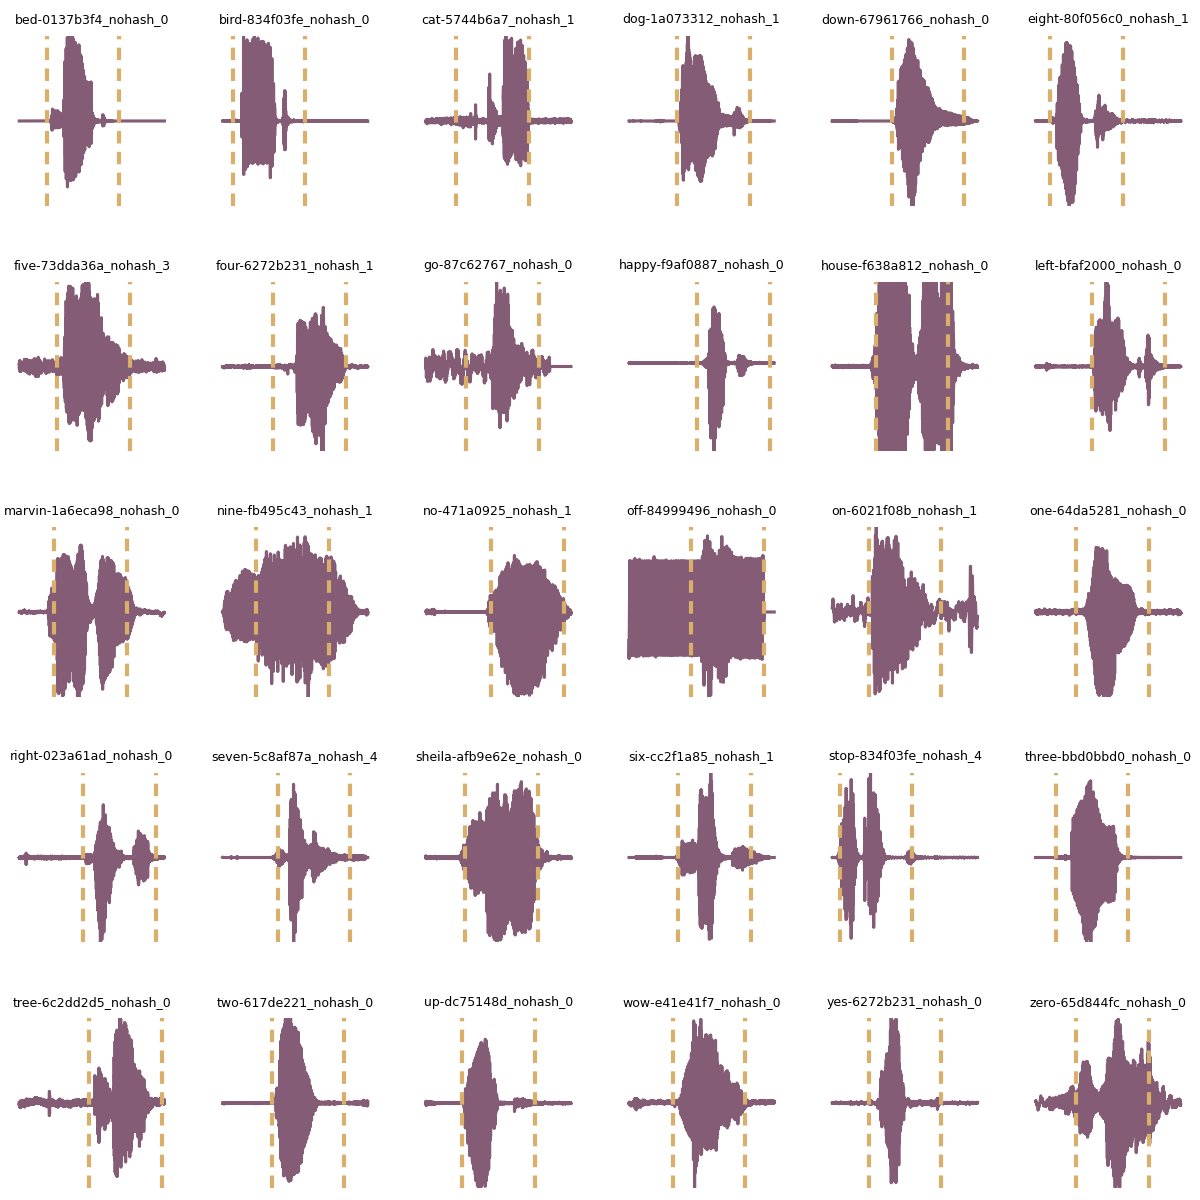
\includegraphics[width=0.65\textwidth]{./5_exp/figs/exp_dataset_wav_grid_c30}
  \caption{One random sample of each individual speech command in the speech command dataset in normalized raw audio format.}
  \label{fig:exp_dataset_wav_grid_c30}
\end{figure}
\FloatBarrier
\noindent

% dataset structure
\subsubsection{Dataset Structure}
The speech command examples are stored in separate folders, named after each individual speech command, in the \texttt{.wav} format.
The folder named as \texttt{\_background\_noise\_} contains six different background noise files, such as \texttt{white\_noise.wav} or \texttt{doing\_the\_dishes.wav}, with a duration of more than one minute each.
Noise examples with a new noise label named \texttt{_noise} were extracted from those background noise files with a \SI{1}{\second} window shifted by \SI{0.2}{\second}.

Each waveform file is named with an 8-digit hexadecimal hash code for the speaker identification, followed by the utterance number, for instance \texttt{3b4f8f24\_nohash\_0.wav}.
Therefore it is possible to distinguish between different speakers, however as mentioned above, no further information about the speaker is given due to data privacy issues.

%It has to be mentioned, that it is wonderful, that a dataset for simple key word spotting on speech commands with this amount of diversity and free of access under the creative common license exist.


% --
% my dataset

\subsection{My own Dataset}\label{sec:exp_dataset_my}
This dataset was created by the author of this thesis and contains five examples samples each from the words \{\enquote{left}, \enquote{right}, \enquote{up}, \enquote{down} and \enquote{go}\}.
The datasets purpose is mainly to have an additional test set for evaluating trained models on the authors own voice with different word pronouncement on each example.
It is important to mention that none of the self recorded files were used within the training set, so that the neural networks performance on this unseen data is evaluated.
All examples of my own dataset are illustrated in \rfig{exp_dataset_wav_grid_my} in raw audio format.
\begin{figure}[!ht]
  \centering
    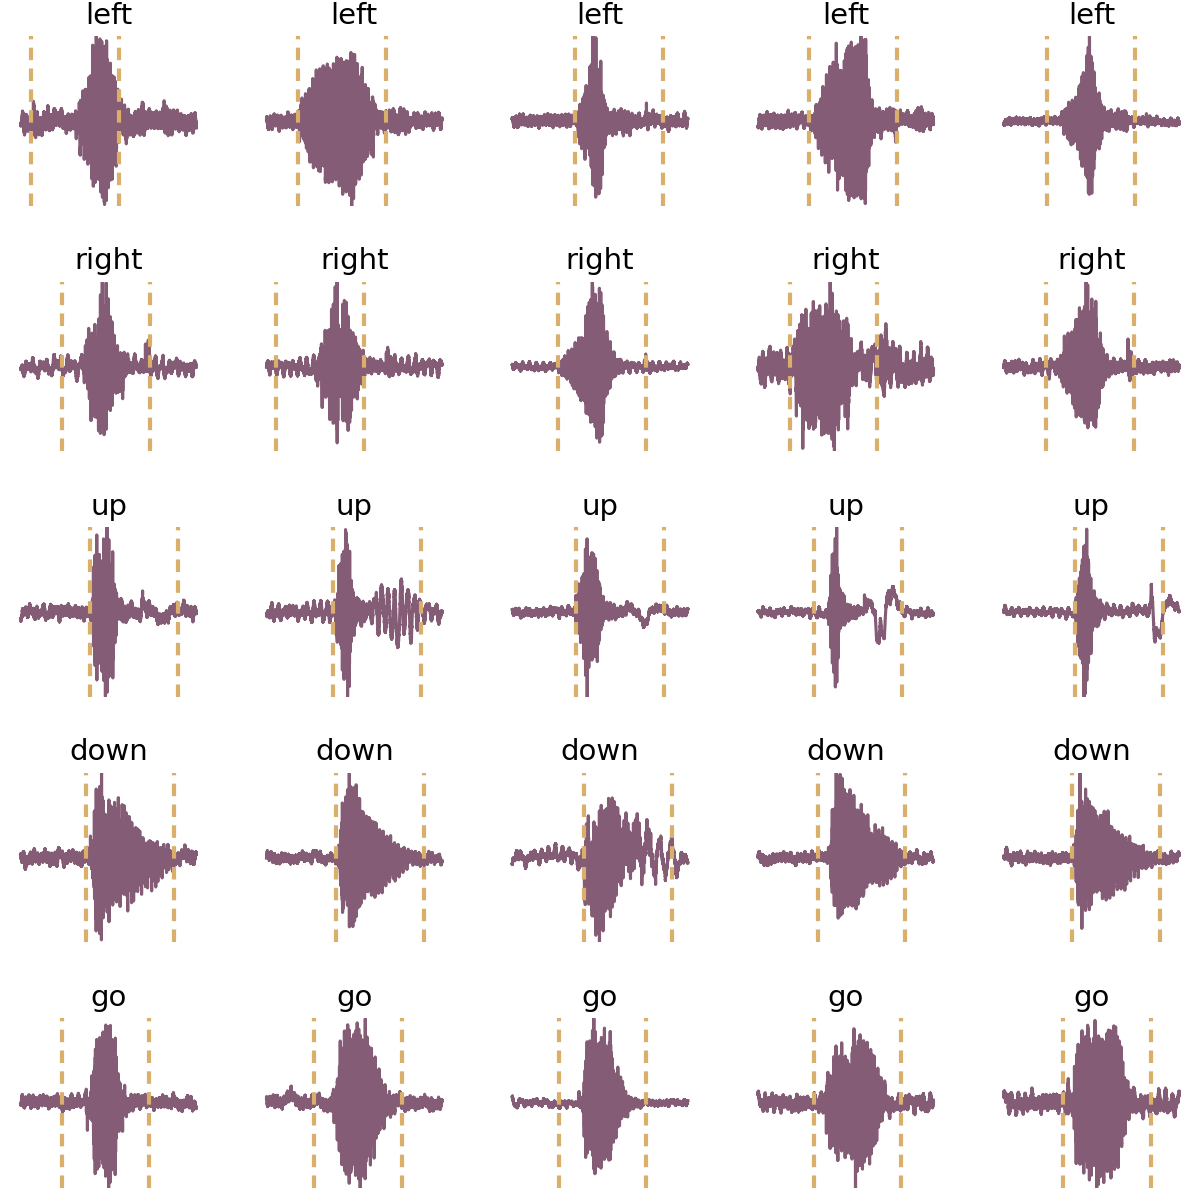
\includegraphics[width=0.65\textwidth]{./5_exp/figs/exp_dataset_wav_grid_my}
  \caption{Self recorded files of the \enquote{my dataset} in raw audio format.}
  \label{fig:exp_dataset_wav_grid_my}
\end{figure}
\FloatBarrier
\noindent
The examples per word are spoken with different emphasis and stress on individual phonemes.
Also the prolongation of the words are different, that in one example the word is fast and in the other its slow spoken.
The emphasis and prolongation ensure the diversity of the dataset. 
It turned out that it is not easy for neural networks to gain a $100\%$ classification score upon it, even though there is only one and the same speaker.



% neural networks
% --
% training details

\section{Implementation and Training Details}\label{sec:exp_details}
In this sections, the implementation und parameters for training are is described in more detail.

\subsection{Implementation notes}\label{sec:exp_details_implementation}
The programming code for this thesis was entirely done in \texttt{Python} with version $>3.8$ evaluated on a linux system.
This might be important if one tries to run the python code on a windows machine, it was not tested for it and could yield in errors (especially regarding paths variables).
For the neural networks implementation and training, the framework \texttt{Pytorch} with version $1.7.0$ was used. 
Usually it should not be a problem if a newer version of \texttt{Pytorch} is applied.
The feature extraction with Mel Frequency Cepstral Coefficients (MFCC) was done with an own implementation, but using efficients functions for transforms functions, such as the short time fourier transform, with packages from \texttt{scipy}.
Matrix computations usually are done with the package \texttt{numpy}.
Several other \texttt{Python} packages were used within the project, but are not named explicitly.


\subsection{Neural Network Training Details}\label{sec:exp_details_training}
We can separate the training details into following parameters to select from:
\begin{enumerate}
  \item Features extraction parameters
  \item Dataset parameters
  \item Feature selection
  \item Transfer Learning parameters
  \item Machine Learning parameters
\end{enumerate}
The feature extraction parameters simply give information about how features are extracted, e.g. this includes the hop size, frame size, filter bands of the MFCC, etc.
The dataset parameters are the information of which labels and how many examples per labels are used
Also they consist of the feature selection, so that the extracted dataset only consists of MFCC data. 
The Abbreviation regarding dataset parameters and feature selection were already listed in \rtab{exp_dataset_abbr}.
%The feature selection is the information about what input feature groups are used in the training, e.g. use cepstral coefficients only, or add delta and energy features, their references are shown in \rtab{dataset_feature_groups}.
The Transfer Learning parameters are pre-trained weights for the actual neural network architecture to be trained.
This could be only the first convolutional layers or entire networks but here all convolutional layers from an adversarial training are considered. 
The Abbreviations for training parameters can be specified as listed in \rtab{exp_details_adv}
\begin{table}[ht!]
\begin{center}
\caption{Adversarial Training abbreviations.}
\begin{tabular}{ M{2cm}  M{5cm} }
\toprule
%\multicolumn{4}{c}{\textbf{Feature Groups}} & \multicolumn{2}{c}{\textbf{Accuracy}} \\
\textbf{Abbreviations} & \textbf{Meaning}\\
\midrule
dec & use of decoder weights\\
enc & use of encoder weights\\
itl[0-9]+ & iterations per label, e.g. itl500 for 500 iterations\\
\bottomrule
\label{tab:exp_details_adv}
\end{tabular}
\end{center}
\end{table}
\FloatBarrier
\noindent


The Machine Learning parameters are classically training parameters such as learning rate, number of epochs, etc.
Their selection and references are listed in \rtab{exp_details_train_params}

\begin{table}[ht!]
\begin{center}
\caption{All training parameters used within this thesis and their abbreviations.}
\begin{tabular}{ M{2cm}  M{5cm} }
\toprule
%\multicolumn{4}{c}{\textbf{Feature Groups}} & \multicolumn{2}{c}{\textbf{Accuracy}} \\
\textbf{Abbreviations} & \textbf{Meaning}\\
\midrule
it[0-9]+ & Number of epochs (or iterations)\\
bs[0-9]+ & Batch size, e.g. bs32 is a batch size of 32 examples\\
lr[0-9.]+ & Learning rate, e.g. lr0.0001\\
mo[0-9.]+ & Momentum, e.g. mo0.5\\
\bottomrule
\label{tab:exp_details_train_params}
\end{tabular}
\end{center}
\end{table}
\FloatBarrier
\noindent


% --
% feature selection

\section{Feature Selection}\label{sec:exp_fs}
The first important Question, when using Neural Networks, is what features are used as inputs.
In the feature extraction section about MFCCs \rsec{signal_mfcc}, it was shown how raw audio files can be extracted to MFCCs and what enhancements can be done.
These enhancements (deltas and energy features) are formed in groups for evaluation to see the impact on the choice and hopefully to reduce the input feature size to a minimum.
%Now that the Neural Network Architectures are described in \rsec{nn_arch} and basic knowledge about MFCCs is given in \rsec{features} it is important to evaluate the impact of the selection of certain MFCC feature constellations to the accuracy of the Test sets.
Beside it is good to get a general overview on what accuracies can be expected from different Neural Network Architectures.
The evaluation is done on 5 classes and 30 classes with different training parameters to observe the impact on a easy and a very hard classification task.
In detail it is shown how models are trained with features consisting of following MFCC groups:
\begin{enumerate}
    \item Cepstral Coefficients (usual MFCCs)
    \item Deltas (frame difference of MFCCs)
    \item Double Deltas (frame difference of Deltas)
    \item Energy Vector (added to each of the upper features)
\end{enumerate}
Another crucial point is to evaluate whether a frame based normalization of these features hurt the training and the accuracy of the models.
Therefore additional columns are presented in the following tables marked with \enquote{norm}.
Note that all these experiments have been done with n-500 a number of 500 examples per class, so that computations are minimized but still enough data is drawn.

\subsection{Feature Selection on Conv Encoder}
The feature selection evaluation on the conv-encoder-fc1 architecture with 5 labels is listed in \rtab{exp_fs_fc1_it500_c5}.
% \begin{table}[ht!]
\begin{center}
\caption{Feature Selection ml it500 c5 features fc1}
\begin{tabular}{ M{1cm}  M{1cm}  M{1cm}  M{1cm}  M{1.5cm}  M{1.5cm}  M{1.5cm}  M{1.5cm} }
\toprule
\multicolumn{4}{c}{\textbf{Feature Groups}} & \multicolumn{2}{c}{\textbf{Accuracy}} \\
\textbf{c} & \textbf{d} & \textbf{dd} & \textbf{e} & \textbf{acc test} & \textbf{acc my} & \textbf{acc test norm} & \textbf{acc my norm} \\
\midrule
0 & 0 & 1 & 0 & 86.67 & 80.00 & 68.33 & 73.33 \\
0 & 0 & 1 & 1 & 85.00 & 86.67 & 67.67 & 73.33 \\
0 & 1 & 0 & 0 & 92.67 & 100.00 & 75.67 & 80.00 \\
0 & 1 & 0 & 1 & 90.67 & 90.00 & 82.00 & 73.33 \\
0 & 1 & 1 & 0 & 91.00 & 93.33 & 76.67 & 70.00 \\
0 & 1 & 1 & 1 & 89.33 & 100.00 & 78.67 & 80.00 \\
1 & 0 & 0 & 0 & 16.67 & 16.67 & 88.33 & 86.67 \\
1 & 0 & 0 & 1 & 33.33 & 33.33 & 86.33 & 80.00 \\
1 & 0 & 1 & 0 & 91.00 & 90.00 & 87.00 & 80.00 \\
1 & 0 & 1 & 1 & 82.67 & 86.67 & 86.67 & 90.00 \\
1 & 1 & 0 & 0 & 91.67 & 76.67 & 88.33 & 90.00 \\
1 & 1 & 0 & 1 & 90.00 & 80.00 & 89.33 & 93.33 \\
1 & 1 & 1 & 0 & 89.00 & 76.67 & 89.33 & 90.00 \\
1 & 1 & 1 & 1 & 88.00 & 90.00 & 89.00 & 86.67 \\
\bottomrule
\end{tabular}
\end{center}
\label{tab:ml_it500_c5_features_fc1}
\end{table}
\FloatBarrier
\noindent


% \begin{table}[ht!]
\begin{center}
\caption{Feature Selection ml it1000 c30 features fc1}
\begin{tabular}{ M{1cm}  M{1cm}  M{1cm}  M{1cm}  M{1.5cm}  M{1.5cm} }
\toprule
\multicolumn{4}{c}{\textbf{Feature Groups}} & \multicolumn{2}{c}{\textbf{Accuracy}} \\
\textbf{c} & \textbf{d} & \textbf{dd} & \textbf{e} & \textbf{acc test} & \textbf{acc test norm} \\
\midrule
0 & 0 & 1 & 0 & 52.97 & 33.10 \\
0 & 0 & 1 & 1 & 56.65 & 27.94 \\
0 & 1 & 0 & 0 & 63.55 & 39.68 \\
0 & 1 & 0 & 1 & 74.52 & 48.65 \\
0 & 1 & 1 & 0 & 71.03 & 39.35 \\
0 & 1 & 1 & 1 & 73.94 & 46.39 \\
1 & 0 & 0 & 0 & 47.23 & 58.19 \\
1 & 0 & 0 & 1 & 45.35 & 57.81 \\
1 & 0 & 1 & 0 & 60.45 & 47.55 \\
1 & 0 & 1 & 1 & 59.48 & 51.61 \\
1 & 1 & 0 & 0 & 58.77 & 55.10 \\
1 & 1 & 0 & 1 & 6.45 & 47.81 \\
1 & 1 & 1 & 0 & 65.81 & 60.39 \\
1 & 1 & 1 & 1 & 62.06 & 51.55 \\
\bottomrule
\end{tabular}
\end{center}
\label{tab:ml_it1000_c30_features_fc1}
\end{table}
\FloatBarrier
\noindent


% \begin{table}[ht!]
\begin{center}
\caption{Feature Selection ml it2000 c30 features fc3}
\begin{tabular}{ M{1cm}  M{1cm}  M{1cm}  M{1cm}  M{1.5cm}  M{1.5cm} }
\toprule
\multicolumn{4}{c}{\textbf{Feature Groups}} & \multicolumn{2}{c}{\textbf{Accuracy}} \\
\textbf{c} & \textbf{d} & \textbf{dd} & \textbf{e} & \textbf{acc test} & \textbf{acc test norm} \\
\midrule
0 & 0 & 1 & 0 & 49.03 & 33.74 \\
0 & 0 & 1 & 1 & 66.90 & 34.84 \\
0 & 1 & 0 & 0 & 77.10 & 55.55 \\
0 & 1 & 0 & 1 & 78.65 & 56.52 \\
0 & 1 & 1 & 0 & 74.97 & 50.26 \\
0 & 1 & 1 & 1 & 73.94 & 59.61 \\
1 & 0 & 0 & 0 & 76.52 & 64.26 \\
1 & 0 & 0 & 1 & 73.87 & 59.16 \\
1 & 0 & 1 & 0 & 78.58 & 63.03 \\
1 & 0 & 1 & 1 & 73.48 & 59.03 \\
1 & 1 & 0 & 0 & 79.10 & 66.13 \\
1 & 1 & 0 & 1 & 80.39 & 60.77 \\
1 & 1 & 1 & 0 & 76.97 & 64.71 \\
1 & 1 & 1 & 1 & 75.94 & 65.55 \\
\bottomrule
\end{tabular}
\end{center}
\label{tab:ml_it2000_c30_features_fc3}
\end{table}
\FloatBarrier
\noindent


\begin{table}[ht!]
\begin{center}
\caption{Feature Selection on arch: conv-encoder-fc1 with dataset: L5-n500 and training params: it500-bs32-lr0.0001-mo0.5}
\begin{tabular}{ M{1cm}  M{1cm}  M{1cm}  M{1cm}  M{1.5cm}  M{1.5cm}  M{1.5cm}  M{1.5cm} }
\toprule
\multicolumn{4}{c}{\textbf{Feature Groups}} & \multicolumn{2}{c}{\textbf{Accuracy}} \\
\textbf{c} & \textbf{d} & \textbf{dd} & \textbf{e} & \textbf{acc test} & \textbf{acc my} & \textbf{acc test norm} & \textbf{acc my norm} \\
\midrule
0 & 0 & 1 & 0 & 86.67 & 80.00 & 68.33 & 73.33 \\
0 & 0 & 1 & 1 & 85.00 & 86.67 & 67.67 & 73.33 \\
0 & 1 & 0 & 0 & 92.67 & 100.00 & 75.67 & 80.00 \\
0 & 1 & 0 & 1 & 90.67 & 90.00 & 82.00 & 73.33 \\
0 & 1 & 1 & 0 & 91.00 & 93.33 & 76.67 & 70.00 \\
0 & 1 & 1 & 1 & 89.33 & 100.00 & 78.67 & 80.00 \\
1 & 0 & 0 & 0 & 16.67 & 16.67 & 88.33 & 86.67 \\
1 & 0 & 0 & 1 & 33.33 & 33.33 & 86.33 & 80.00 \\
1 & 0 & 1 & 0 & 91.00 & 90.00 & 87.00 & 80.00 \\
1 & 0 & 1 & 1 & 82.67 & 86.67 & 86.67 & 90.00 \\
1 & 1 & 0 & 0 & 91.67 & 76.67 & 88.33 & 90.00 \\
1 & 1 & 0 & 1 & 90.00 & 80.00 & 89.33 & 93.33 \\
1 & 1 & 1 & 0 & 89.00 & 76.67 & 89.33 & 90.00 \\
1 & 1 & 1 & 1 & 88.00 & 90.00 & 89.00 & 86.67 \\
\bottomrule
\label{tab:exp_fs_fc1_it500_c5}
\end{tabular}
\end{center}
\end{table}
\FloatBarrier
\noindent


\begin{table}[ht!]
\begin{center}
\caption{Feature Selection on arch: conv-encoder-fc1 with dataset: L30-n500 and training params: it1000-bs128-lr0.0001-mo0.5}
\begin{tabular}{ M{1cm}  M{1cm}  M{1cm}  M{1cm}  M{1.5cm}  M{1.5cm} }
\toprule
\multicolumn{4}{c}{\textbf{Feature Groups}} & \multicolumn{2}{c}{\textbf{Accuracy}} \\
\textbf{c} & \textbf{d} & \textbf{dd} & \textbf{e} & \textbf{acc test} & \textbf{acc test norm} \\
\midrule
0 & 0 & 1 & 0 & 52.97 & 33.10 \\
0 & 0 & 1 & 1 & 56.65 & 27.94 \\
0 & 1 & 0 & 0 & 63.55 & 39.68 \\
0 & 1 & 0 & 1 & 74.52 & 48.65 \\
0 & 1 & 1 & 0 & 71.03 & 39.35 \\
0 & 1 & 1 & 1 & 73.94 & 46.39 \\
1 & 0 & 0 & 0 & 47.23 & 58.19 \\
1 & 0 & 0 & 1 & 45.35 & 57.81 \\
1 & 0 & 1 & 0 & 60.45 & 47.55 \\
1 & 0 & 1 & 1 & 59.48 & 51.61 \\
1 & 1 & 0 & 0 & 58.77 & 55.10 \\
1 & 1 & 0 & 1 & 6.45 & 47.81 \\
1 & 1 & 1 & 0 & 65.81 & 60.39 \\
1 & 1 & 1 & 1 & 62.06 & 51.55 \\
\bottomrule
\label{tab:exp_fs_fc1_it1000_c30}
\end{tabular}
\end{center}
\end{table}
\FloatBarrier
\noindent


\begin{table}[ht!]
\begin{center}
\caption{Feature Selection on arch: conv-encoder-fc3 with dataset: L30-n500 and training params: it2000-bs128-lr0.0001-mo0.5}
\begin{tabular}{ M{1cm}  M{1cm}  M{1cm}  M{1cm}  M{1.5cm}  M{1.5cm} }
\toprule
\multicolumn{4}{c}{\textbf{Feature Groups}} & \multicolumn{2}{c}{\textbf{Accuracy}} \\
\textbf{c} & \textbf{d} & \textbf{dd} & \textbf{e} & \textbf{acc test} & \textbf{acc test norm} \\
\midrule
0 & 0 & 1 & 0 & 49.03 & 33.74 \\
0 & 0 & 1 & 1 & 66.90 & 34.84 \\
0 & 1 & 0 & 0 & 77.10 & 55.55 \\
0 & 1 & 0 & 1 & 78.65 & 56.52 \\
0 & 1 & 1 & 0 & 74.97 & 50.26 \\
0 & 1 & 1 & 1 & 73.94 & 59.61 \\
1 & 0 & 0 & 0 & 76.52 & 64.26 \\
1 & 0 & 0 & 1 & 73.87 & 59.16 \\
1 & 0 & 1 & 0 & 78.58 & 63.03 \\
1 & 0 & 1 & 1 & 73.48 & 59.03 \\
1 & 1 & 0 & 0 & 79.10 & 66.13 \\
1 & 1 & 0 & 1 & 80.39 & 60.77 \\
1 & 1 & 1 & 0 & 76.97 & 64.71 \\
1 & 1 & 1 & 1 & 75.94 & 65.55 \\
\bottomrule
\label{tab:exp_fs_fc3_it2000_c30}
\end{tabular}
\end{center}
\end{table}
\FloatBarrier
\noindent



\subsection{Feature Selection on fstride}
fstride
\begin{table}[ht!]
\begin{center}
\caption{Feature Selection on arch: conv-fstride with dataset: L5-n500 and training params: it1000-bs32-lr0.0001-mo0.5}
\begin{tabular}{ M{1cm}  M{1cm}  M{1cm}  M{1cm}  M{1.5cm}  M{1.5cm}  M{1.5cm}  M{1.5cm} }
\toprule
\multicolumn{4}{c}{\textbf{Feature Groups}} & \multicolumn{2}{c}{\textbf{Accuracy}} \\
\textbf{c} & \textbf{d} & \textbf{dd} & \textbf{e} & \textbf{acc test} & \textbf{acc my} & \textbf{acc test norm} & \textbf{acc my norm} \\
\midrule
0 & 0 & 1 & 0 & 65.67 & 56.67 & 43.67 & 53.33 \\
0 & 0 & 1 & 1 & 64.33 & 60.00 & 49.00 & 43.33 \\
0 & 1 & 0 & 0 & 86.00 & 83.33 & 69.00 & 63.33 \\
0 & 1 & 0 & 1 & 85.00 & 76.67 & 67.67 & 83.33 \\
0 & 1 & 1 & 0 & 84.67 & 76.67 & 72.33 & 73.33 \\
0 & 1 & 1 & 1 & 84.00 & 80.00 & 76.00 & 66.67 \\
1 & 0 & 0 & 0 & 88.33 & 76.67 & 84.33 & 73.33 \\
1 & 0 & 0 & 1 & 90.00 & 86.67 & 81.67 & 70.00 \\
1 & 0 & 1 & 0 & 89.00 & 80.00 & 86.00 & 86.67 \\
1 & 0 & 1 & 1 & 88.67 & 83.33 & 83.67 & 80.00 \\
1 & 1 & 0 & 0 & 89.33 & 83.33 & 86.33 & 73.33 \\
1 & 1 & 0 & 1 & 90.00 & 80.00 & 86.67 & 80.00 \\
1 & 1 & 1 & 0 & 89.00 & 76.67 & 86.33 & 73.33 \\
1 & 1 & 1 & 1 & 90.67 & 86.67 & 86.00 & 86.67 \\
\bottomrule
\label{tab:exp_fs_fstride_it1000_c5}
\end{tabular}
\end{center}
\end{table}
\FloatBarrier
\noindent



\subsection{Feature Selection on trad}
trad
\begin{table}[ht!]
\begin{center}
\caption{Feature Selection on arch: conv-trad with dataset: L5-n500 and training params: it1000-bs32-lr0.0001-mo0.5}
\begin{tabular}{ M{1cm}  M{1cm}  M{1cm}  M{1cm}  M{1.5cm}  M{1.5cm}  M{1.5cm}  M{1.5cm} }
\toprule
\multicolumn{4}{c}{\textbf{Feature Groups}} & \multicolumn{2}{c}{\textbf{Accuracy}} \\
\textbf{c} & \textbf{d} & \textbf{dd} & \textbf{e} & \textbf{acc test} & \textbf{acc my} & \textbf{acc test norm} & \textbf{acc my norm} \\
\midrule
0 & 0 & 1 & 0 & 84.00 & 86.67 & 65.33 & 56.67 \\
0 & 0 & 1 & 1 & 85.67 & 86.67 & 72.00 & 66.67 \\
0 & 1 & 0 & 0 & 91.67 & 83.33 & 84.67 & 66.67 \\
0 & 1 & 0 & 1 & 93.33 & 93.33 & 83.33 & 80.00 \\
0 & 1 & 1 & 0 & 93.33 & 86.67 & 86.33 & 80.00 \\
0 & 1 & 1 & 1 & 91.67 & 90.00 & 90.33 & 80.00 \\
1 & 0 & 0 & 0 & 94.33 & 93.33 & 92.00 & 83.33 \\
1 & 0 & 0 & 1 & 95.00 & 90.00 & 91.00 & 93.33 \\
1 & 0 & 1 & 0 & 93.67 & 90.00 & 94.67 & 83.33 \\
1 & 0 & 1 & 1 & 91.67 & 96.67 & 94.00 & 76.67 \\
1 & 1 & 0 & 0 & 95.00 & 83.33 & 92.67 & 83.33 \\
1 & 1 & 0 & 1 & 94.67 & 93.33 & 92.00 & 86.67 \\
1 & 1 & 1 & 0 & 95.33 & 90.00 & 92.00 & 86.67 \\
1 & 1 & 1 & 1 & 95.00 & 100.00 & 94.00 & 86.67 \\
\bottomrule
\label{tab:exp_fs_trad_it1000_c5}
\end{tabular}
\end{center}
\end{table}
\FloatBarrier
\noindent




% --
% adversarial training

\section{Adversarial Training}\label{sec:exp_adv}
\thesisStateNotReady
Here the Adversarial Training is evalutated.
The first comparance is between a the conv-encoder-fc3 once with adversarial init (use of) and once with simple random init.
The training losses of those two methods are shown in \rfig{exp_adv_fc3_train_loss} and their accuracies in \rfig{exp_adv_fc3_val_acc}.

\begin{figure}[!ht]
  \centering
    \subfigure[adv init]{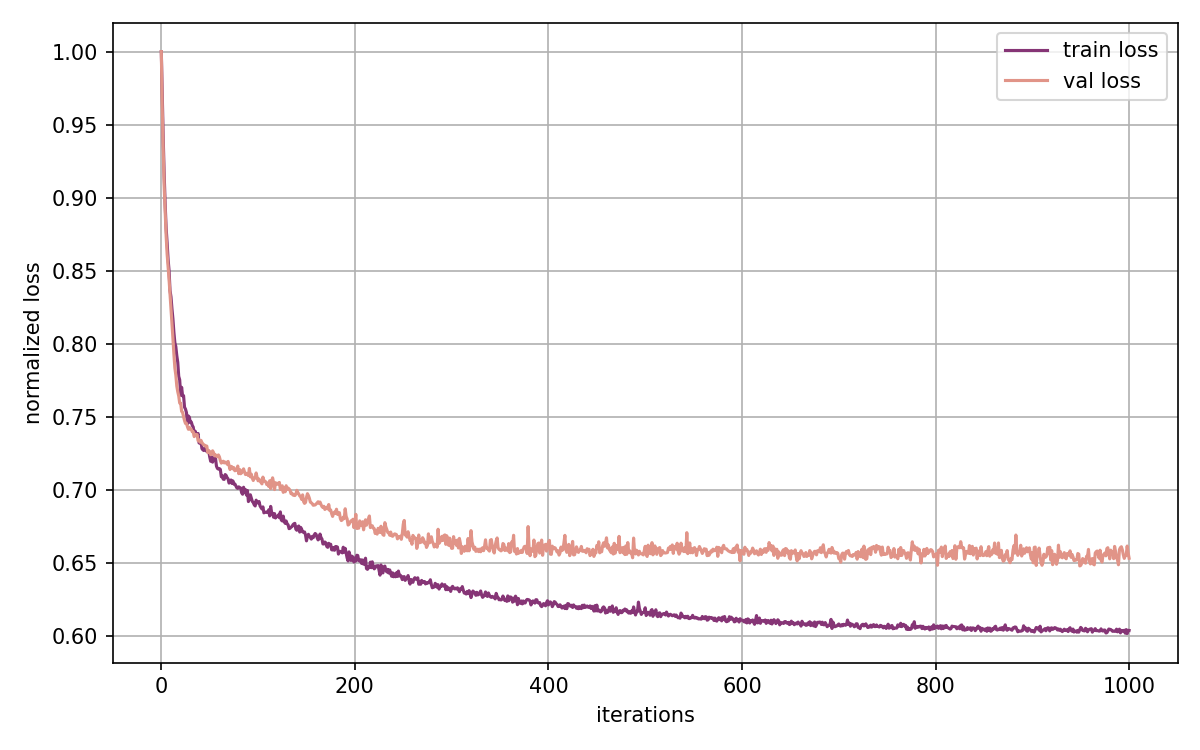
\includegraphics[width=0.45\textwidth]{./5_exp/figs/exp_adv_fc3_train_loss_label}}
    \subfigure[random init]{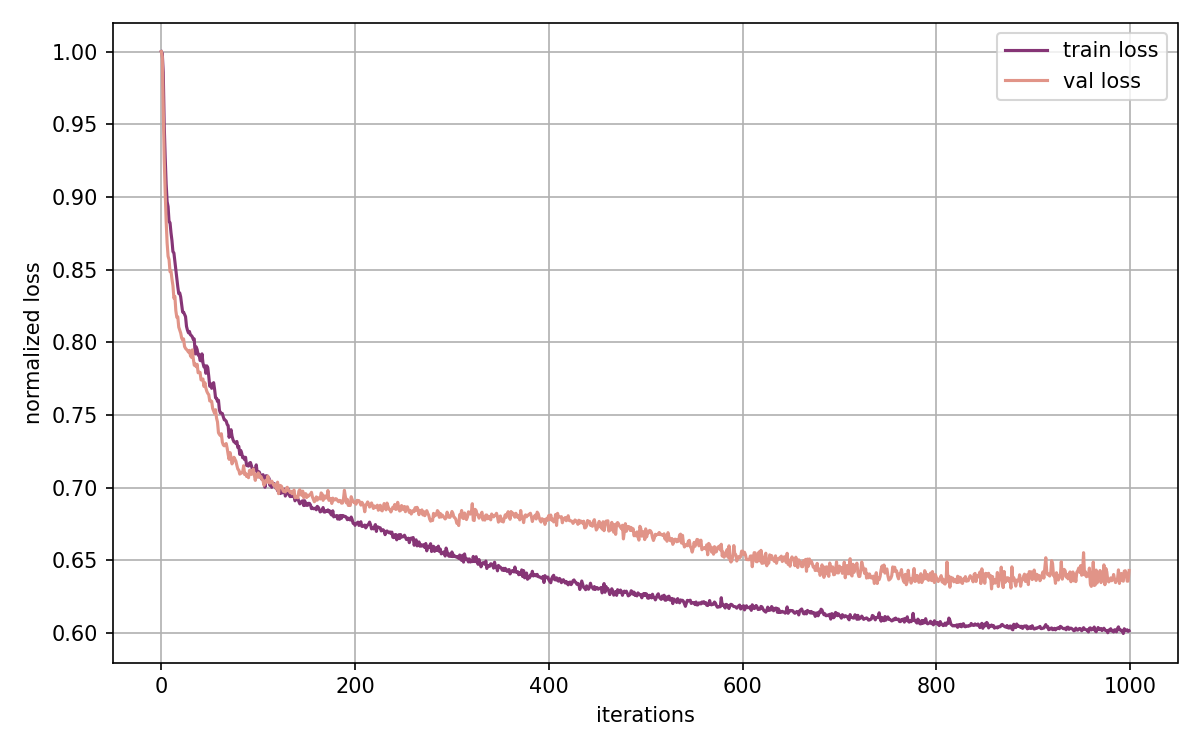
\includegraphics[width=0.45\textwidth]{./5_exp/figs/exp_adv_fc3_train_loss_random}}
  \caption{Comparing the train loss of L5-n500-norm1, c1d0dd0e0-norm1-it1000-bs32-lr0.0001-mo0.5 once with random init and once with adv init with dec-itl1000.}
  \label{fig:exp_adv_fc3_train_loss}
\end{figure}
\FloatBarrier
\noindent

\begin{figure}[!ht]
  \centering
    \subfigure[adv init]{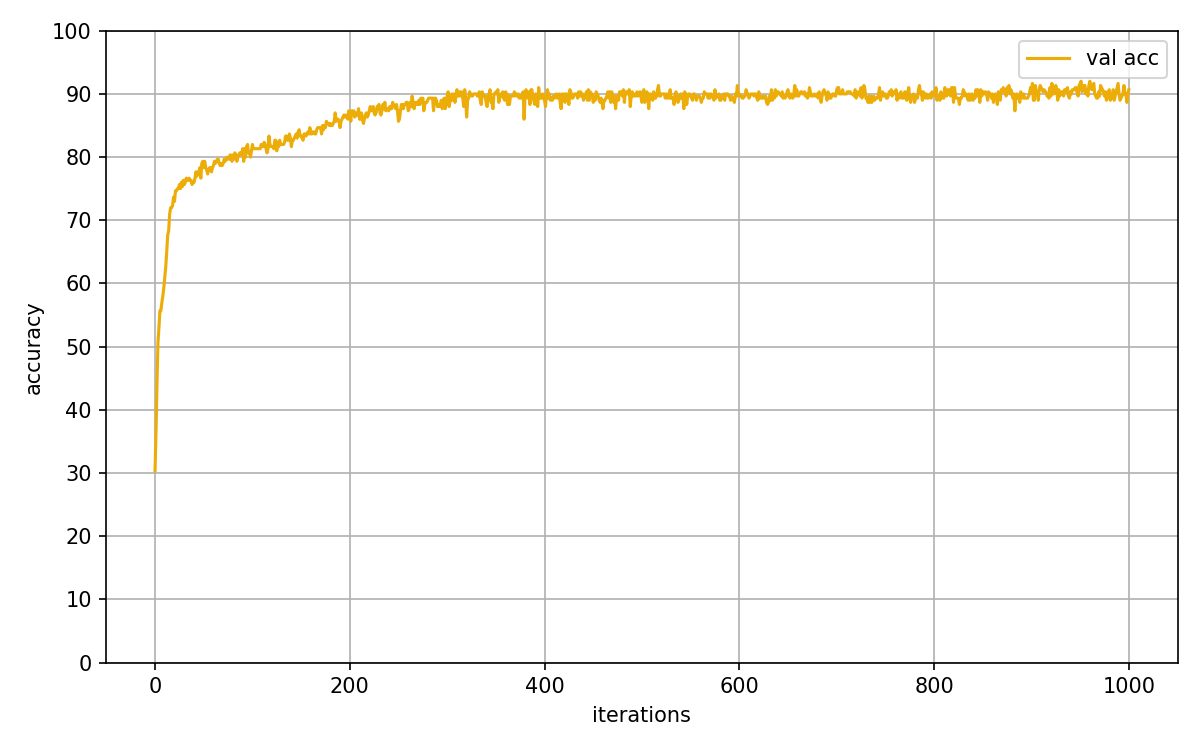
\includegraphics[width=0.45\textwidth]{./5_exp/figs/exp_adv_fc3_val_acc_label}}
    \subfigure[random init]{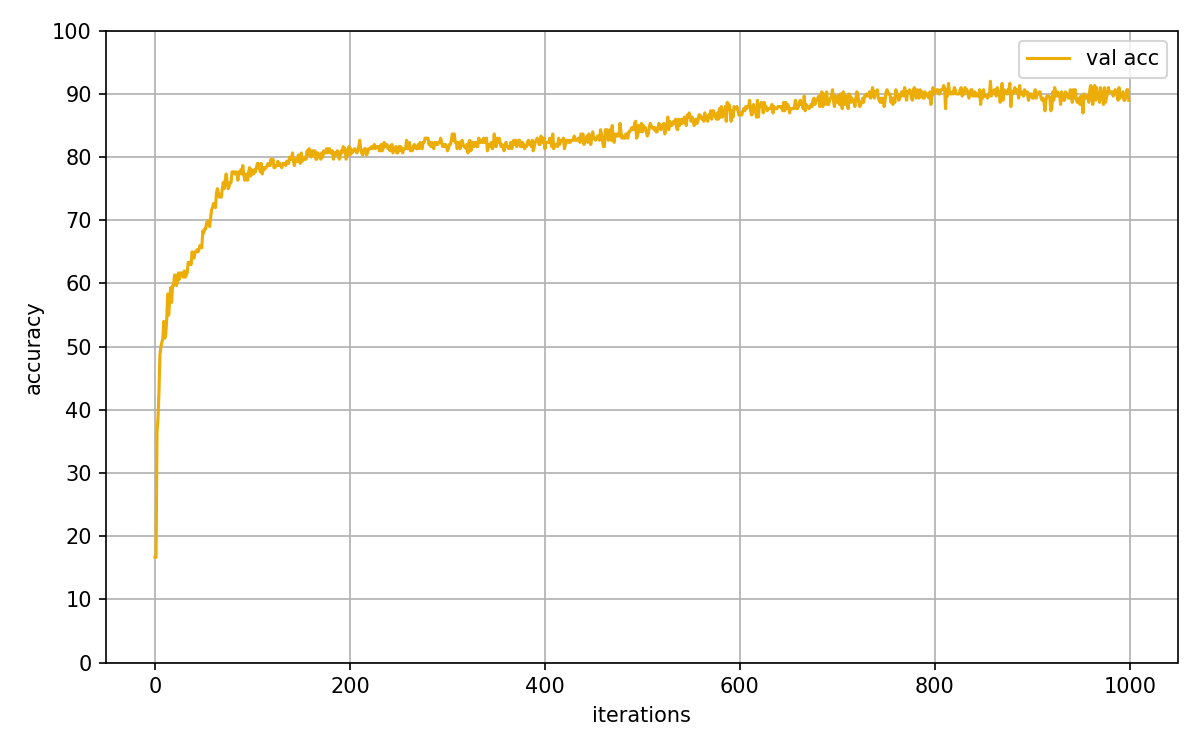
\includegraphics[width=0.45\textwidth]{./5_exp/figs/exp_adv_fc3_val_acc_random}}
  \caption{Comparing the validation accuracy of L5-n500, c1d0dd0e0-norm1-it1000-bs32-lr0.0001-mo0.5 once with random init and once with adv init with dec-itl1000.}
  \label{fig:exp_adv_fc3_val_acc}
\end{figure}
\FloatBarrier
\noindent

The loss and accuracy plots show how well the training was going forward for this showcase example. Both training work well and seem to converge, the one of the adversarial init parameters has a considerably faster convergence time here than the one without.
The scores on the test sets are shown in \rtab{exp_adv_fc3_score}, where both are achieving high scores on the test set, while the adversarial init one got a few percent more, but less on the my set.
This does not necessarily proof if one method is better or worse, therefore a more challenging task must be picked.
But at least it shows that adversarial pre training works at least as good as random initialization.
\begin{table}[ht!]
\begin{center}
\caption{Score comparison on arch: conv-encoder-fc3 with dataset: L5-n500 and training params: c1d0dd0e0-norm1-it1000-bs32-lr0.0001-mo0.5 and different adv params.}
\begin{tabular}{ M{2cm}  M{1.5cm}  M{1.5cm} }
\toprule
\textbf{adv params} & \textbf{acc test} & \textbf{acc my} \\
\midrule
none & 88.33 & 93.33 \\
dec-itl-1000 & 91.67 & 90.00 \\
\bottomrule
\label{tab:exp_adv_fc3_score}
\end{tabular}
\end{center}
\end{table}
\FloatBarrier
\noindent


\subsection{Wavenets}
Wavenets...
% --
% test bench

\section{Test Bench of best Neural Network Architectures}\label{sec:exp_tb}
\thesisStateNotReady
This section compares the best neural network architectures in terms of noise and shift invariance to fixed self recorded test audio files of the five speech commands with L5 labels.
The length of those audio files is cut, such that by applying a the fixed input frames of \SI{500}{\milli\second}, both end positions consists of at least the half of the audio file information.
This is especially important for the shift invariance.
The noise invariance finds the highest energy region, as described in \rsec{signal_raw} and uses this frame for classification.

% --
% shift invariance

\subsection{Shift invariances}
Shift invariances is very important for speech recognition, for instance the waveform should still be classified to the same class, when shifted a little bit in time.
However the restricted frame size of \SI{500}{\milli\second} makes this task very difficult, as it is already known that not all information might fit into the analytic window, like the \enquote{t} in \enquote{left} or \enquote{right} is often missed.
The figures in this section present a correct classification with a colored pixel and an incorrect with a white pixel.
The examples from the adversarial training section are shown in \rfig{exp_tb_shift_fc3}.
\begin{figure}[!ht]
  \centering
    \subfigure[adv init]{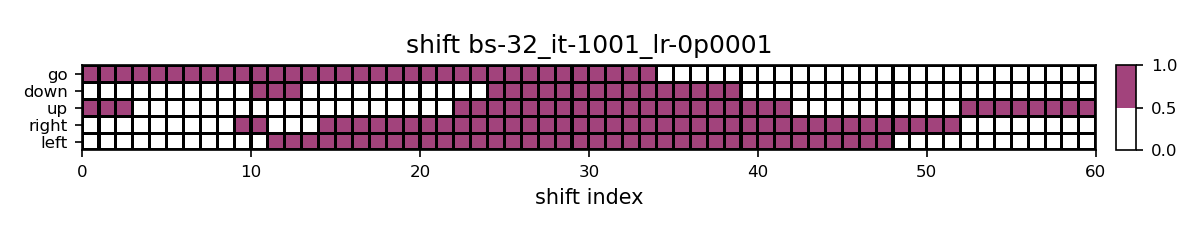
\includegraphics[width=0.45\textwidth]{./5_exp/figs/exp_tb_shift_fc3_adv}}
    \subfigure[random init]{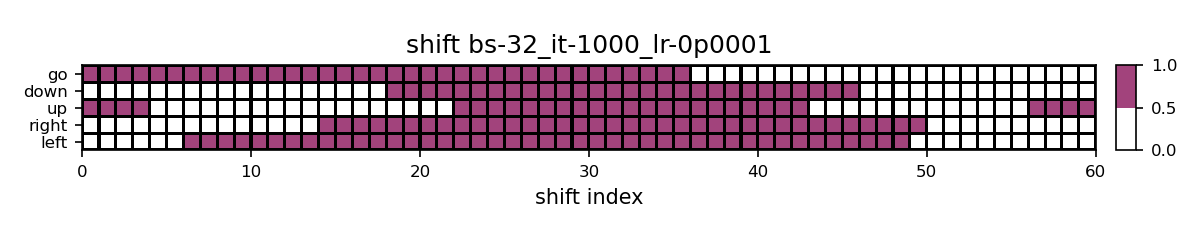
\includegraphics[width=0.45\textwidth]{./5_exp/figs/exp_tb_shift_fc3_random}}
  \caption{Shift invariance of L5-n500, c1d0dd0e0-norm1-it1000-bs32-lr0.0001-mo0.5 once with random init and once with adv init with dec-itl1000.}
  \label{fig:exp_tb_shift_fc3}
\end{figure}
\FloatBarrier
\noindent


% --
% noise invariance

\subsection{Noise invariances}
Noise invariance is a good trait in the classification of speech signals.
That is because the usage of bad microphones or recording set ups may add a lot of noise to the audio and therefore might disturb the classification accuracy.
To create a test upon noise invariance, artificial normal noise is added to the test audio files.
In the plots this is indicated in the x-axis of the plots as Signal to Noise Ration (SNR).
A SNR level of zero means there is equal energy of noise and signal, therefore this signal is already pretty much disturbed.
\rfig{exp_tb_noise_fc3} shows the noise invariance from the example in the adversarial training section.

\begin{figure}[!ht]
  \centering
    \subfigure[adv init]{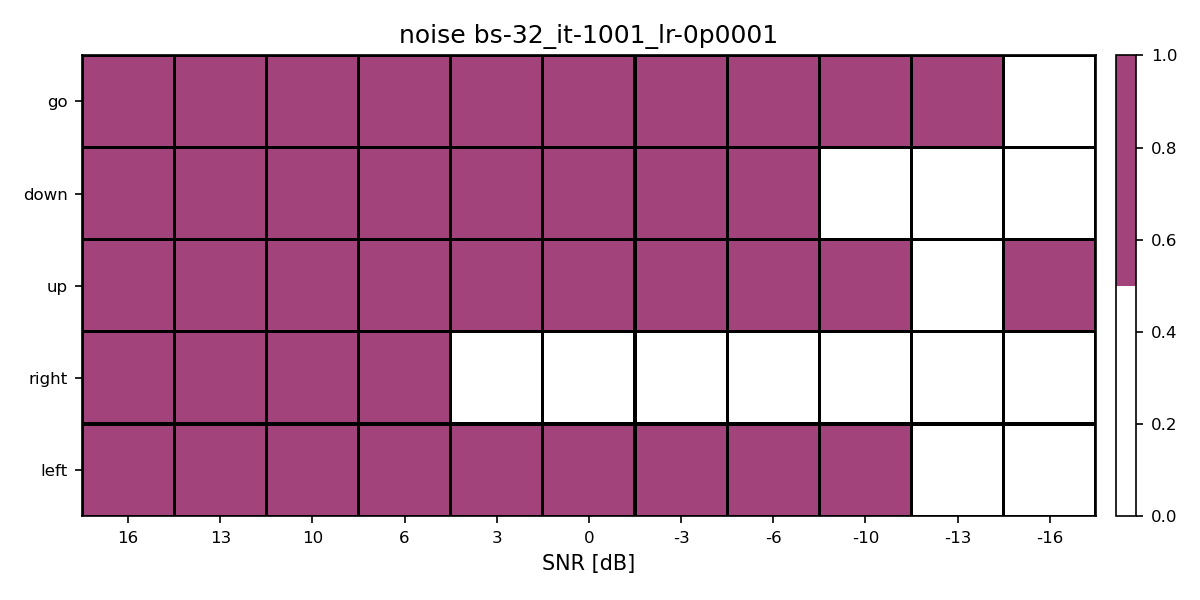
\includegraphics[width=0.40\textwidth]{./5_exp/figs/exp_tb_noise_fc3_adv}}
    \subfigure[random init]{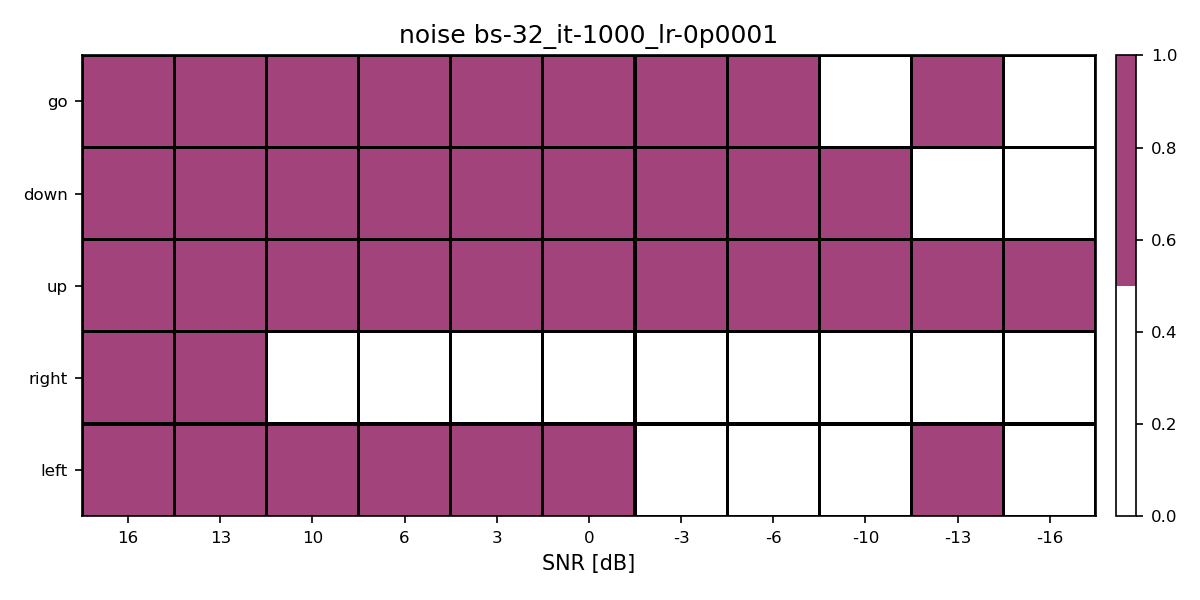
\includegraphics[width=0.40\textwidth]{./5_exp/figs/exp_tb_noise_fc3_random}}
  \caption{Noise invariance of L5-n500, c1d0dd0e0-norm1-it1000-bs32-lr0.0001-mo0.5 once with random init and once with adv init with dec-itl1000.}
  \label{fig:exp_tb_noise_fc3}
\end{figure}
\FloatBarrier
\noindent


